\item[8] Design a Deterministic Finite-state automaton (DFA)  that accepts  exactly the
  strings over the  alphabet $\{ \verb@A@, \verb@B@, \ldots, \verb@Z@  \}$ that
  \begin{itemize}
      \item must contain "NG",
      \item does not end with Y,
      \item any I it contains must be followed by a S (after any number of other letters including another I).
  \end{itemize}
  For instance, your DFA should accept the strings
  \begin{itemize}
  \item STRINGS
  \item VAINGLORIOUS
  \item ENGINEERS
  \item MONOPHTHONG
  \end{itemize}
  but not the strings
  \begin{itemize}
  \item TREPIDATIOUS (does not contain NG).
  \item INDISTINGUISHABLY (ends with a Y).
  \item FINGERPRINT (contains an I that is not followed by S).
  \item INQUISITIVELY (violates all rules).
  \end{itemize}
  You \textbf{must} describe the  meaning of each state in your DFA.
  
  Hint: there is a solution with 14 states, although having additional garbage states (non-accepting states where every outgoing edge loops back to that state) may help with readability.
  \\{\color{NavyBlue}
  \\ Here is a DFA that works. We used 12 states just like the hint states. We have three conditions to check for. Here are the ideas:
  
\begin{itemize}
  \item  If there is "Y" as input after it's reach accepting state and no input afterwards, then it goes to a non-accepting state. This is represented by the "Y" arrow from S2 to S7. If the string is not already at accepting, then it's not accepting whether or not it ends with "Y", so there doesn't need to be a Y state for all individual states. Additionally, there is no way to get into accepting with "Y", so we don't have to worry about that.
  \item "NG" must be in this particular order, so if an input after "N" is not "G", we must go back to the previous state. This is represented by the "else" arrows from S5 and S1, where the input to get to that state is "N". 
  \item If there's "I", then "S" has to exist. Since "NG" has to exist to get to accepting state, it can be before any "I" then "S" [1], in between "I" and "S" [2], after "I" then "S" [3], or "I" then "S" can not exist at all [4]. The first three cases can have overlaps. For example, you can overlap [1] and [2] by after "I" then "S" after and bofore "NG". We can break these 4 cases into parts of the diagram. The order of the states presented are according to which state will be traveled to first. In explained order, [1] is represented by S0, S4, S1, S2; [2] by S0, S4, S5, S6, S2; by [3] is S0, S1, S2, S3; [4] by S0, S1, S2.
  \end{itemize}
  \\
  }

\begin{center}
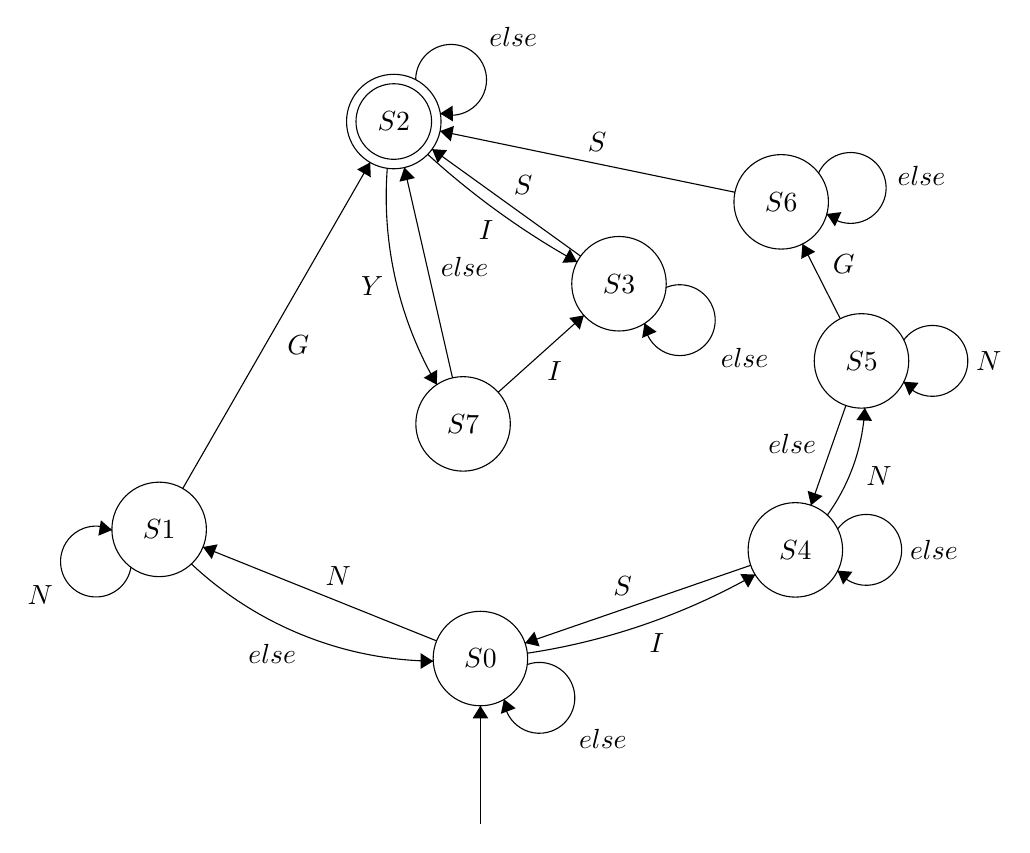
\begin{tikzpicture}[scale=0.2]
\tikzstyle{every node}+=[inner sep=0pt]
\draw [black] (34.4,-42.3) circle (3);
\draw (34.4,-42.3) node {$S0$};
\draw [black] (14,-34.1) circle (3);
\draw (14,-34.1) node {$S1$};
\draw [black] (28.9,-8.2) circle (3);
\draw (28.9,-8.2) node {$S2$};
\draw [black] (28.9,-8.2) circle (2.4);
\draw [black] (43.2,-18.5) circle (3);
\draw (43.2,-18.5) node {$S3$};
\draw [black] (54.4,-35.4) circle (3);
\draw (54.4,-35.4) node {$S4$};
\draw [black] (58.6,-23.4) circle (3);
\draw (58.6,-23.4) node {$S5$};
\draw [black] (33.3,-27.4) circle (3);
\draw (33.3,-27.4) node {$S7$};
\draw [black] (53.5,-13.3) circle (3);
\draw (53.5,-13.3) node {$S6$};
\draw [black] (34.4,-52.8) -- (34.4,-45.3);
\fill [black] (34.4,-45.3) -- (33.9,-46.1) -- (34.9,-46.1);
\draw [black] (40.538,-17.118) arc (-119.1334:-132.39549:50.606);
\fill [black] (40.54,-17.12) -- (40.08,-16.29) -- (39.6,-17.17);
\draw (34.76,-14.47) node [below] {$I$};
\draw [black] (31.62,-41.18) -- (16.78,-35.22);
\fill [black] (16.78,-35.22) -- (17.34,-35.98) -- (17.71,-35.05);
\draw (25.37,-37.68) node [above] {$N$};
\draw [black] (15.5,-31.5) -- (27.4,-10.8);
\fill [black] (27.4,-10.8) -- (26.57,-11.24) -- (27.44,-11.74);
\draw (22.11,-22.38) node [right] {$G$};
\draw [black] (51.845,-36.971) arc (-60.45788:-81.47325:41.953);
\fill [black] (51.85,-36.97) -- (50.9,-36.93) -- (51.4,-37.8);
\draw (45.6,-40.66) node [below] {$I$};
\draw [black] (58.81,-26.386) arc (-2.75892:-35.82117:12.681);
\fill [black] (58.81,-26.39) -- (58.27,-27.16) -- (59.27,-27.21);
\draw (58.87,-30.71) node [right] {$N$};
\draw [black] (31.634,-24.908) arc (-149.85136:-184.33382:23.777);
\fill [black] (31.63,-24.91) -- (31.66,-23.96) -- (30.8,-24.47);
\draw (28.27,-18.67) node [left] {$Y$};
\draw [black] (30.289,-5.554) arc (180.02737:-107.97263:2.25);
\draw (34.94,-2.85) node [right] {$else$};
\fill [black] (31.85,-7.69) -- (32.65,-8.19) -- (32.64,-7.19);
\draw [black] (57.08,-34.077) arc (144:-144:2.25);
\draw (61.65,-35.4) node [right] {$else$};
\fill [black] (57.08,-36.72) -- (57.43,-37.6) -- (58.02,-36.79);
\draw [black] (37.363,-42.686) arc (110.30993:-177.69007:2.25);
\draw (40.63,-47.38) node [right] {$else$};
\fill [black] (35.9,-44.89) -- (35.7,-45.81) -- (36.64,-45.46);
\draw [black] (57.25,-20.72) -- (54.85,-15.98);
\fill [black] (54.85,-15.98) -- (54.77,-16.92) -- (55.66,-16.47);
\draw (56.74,-17.23) node [right] {$G$};
\draw [black] (50.56,-12.69) -- (31.84,-8.81);
\fill [black] (31.84,-8.81) -- (32.52,-9.46) -- (32.72,-8.48);
\draw (41.82,-10.16) node [above] {$S$};
\draw [black] (55.868,-11.478) arc (155.30993:-132.69007:2.25);
\draw (60.86,-11.66) node [right] {$else$};
\fill [black] (56.39,-14.07) -- (56.91,-14.86) -- (57.32,-13.95);
\draw [black] (57.61,-26.23) -- (55.39,-32.57);
\fill [black] (55.39,-32.57) -- (56.13,-31.98) -- (55.18,-31.65);
\draw (55.74,-28.65) node [left] {$else$};
\draw [black] (40.77,-16.75) -- (31.33,-9.95);
\fill [black] (31.33,-9.95) -- (31.69,-10.83) -- (32.28,-10.02);
\draw (37.11,-12.85) node [above] {$S$};
\draw [black] (31.407,-42.466) arc (-90.59809:-133.1983:22.788);
\fill [black] (31.41,-42.47) -- (30.61,-41.96) -- (30.6,-42.96);
\draw (21.18,-41.36) node [below] {$else$};
\draw [black] (51.56,-36.38) -- (37.24,-41.32);
\fill [black] (37.24,-41.32) -- (38.16,-41.53) -- (37.83,-40.59);
\draw (43.44,-38.32) node [above] {$S$};
\draw [black] (12.211,-36.494) arc (-9.03776:-297.03776:2.25);
\draw (7.29,-38.28) node [left] {$N$};
\fill [black] (11.01,-34.14) -- (10.3,-33.52) -- (10.14,-34.5);
\draw [black] (61.28,-22.077) arc (144:-144:2.25);
\draw (65.85,-23.4) node [right] {$N$};
\fill [black] (61.28,-24.72) -- (61.63,-25.6) -- (62.22,-24.79);
\draw [black] (32.63,-24.48) -- (29.57,-11.12);
\fill [black] (29.57,-11.12) -- (29.26,-12.02) -- (30.24,-11.79);
\draw (31.85,-17.4) node [right] {$else$};
\draw [black] (35.53,-25.39) -- (40.97,-20.51);
\fill [black] (40.97,-20.51) -- (40.04,-20.67) -- (40.71,-21.41);
\draw (39.1,-23.44) node [below] {$I$};
\draw [black] (46.178,-18.743) arc (113.0634:-174.9366:2.25);
\draw (49.63,-23.23) node [right] {$else$};
\fill [black] (44.82,-21.01) -- (44.67,-21.94) -- (45.59,-21.55);
\end{tikzpicture}
\end{center}

\\
